\hypertarget{results}{%
\section{Results}\label{results}}

\hypertarget{the-ground-state}{%
\subsection{The Ground State}\label{the-ground-state}}

\begin{figure}
\hypertarget{fig:fermion_gap_vs_L}{%
\centering
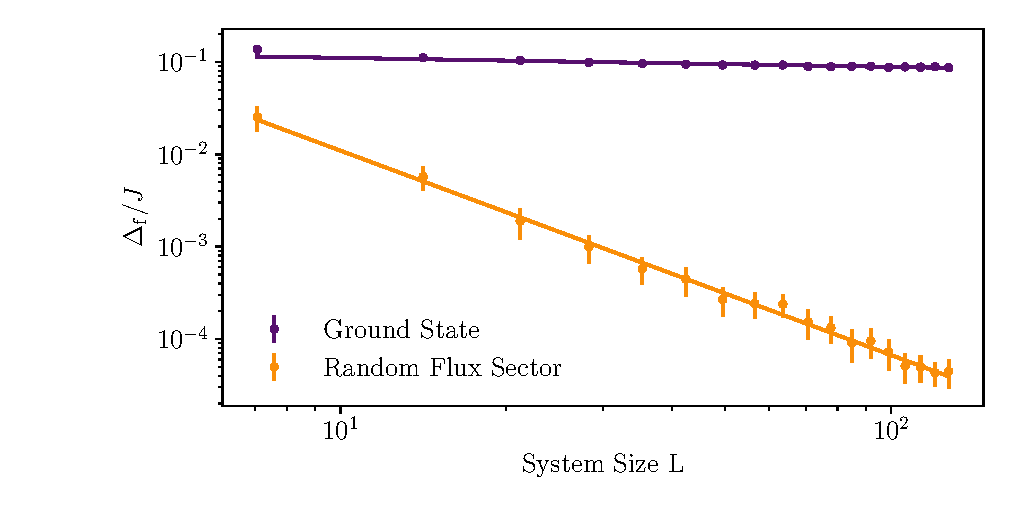
\includegraphics[width=1\textwidth,height=\textheight]{figure_code/amk_chapter/results/fermion_gap_vs_L/fermion_gap_vs_L.pdf}
\caption{Within a flux sector, the fermion gap \(\Delta_f\) measures the
energy between the fermionic ground state and the first excited state.
This graph shows the fermion gap as a function of system size for the
ground state flux sector and for a configuration of random fluxes. We
see that the disorder induced by an putting the Kitaev model on an
amorphous lattice does not close the gap in the ground state. The gap
closes in the flux disordered limit is good evidence that the system
transitions to a gapless thermal metal state at high temperature. Each
point shows an average over 100 lattice realisations. System size \(L\)
is defined \(\sqrt{N}\) where N is the number of plaquettes in the
system. Error bars shown are \(3\) times the standard error of the mean.
The lines shown are fits of \(\tfrac{\Delta_f}{J} = aL ^ b\) with fit
parameters: Ground State: \(a = 0.138 \pm 0.002, b = -0.0972 \pm 0.004\)
Random Flux Sector:
\(a = 1.8 \pm 0.2, b = -2.21 \pm 0.03\)}\label{fig:fermion_gap_vs_L}
}
\end{figure}

\hypertarget{ground-state-phase-diagram}{%
\subsection{Ground State Phase
Diagram}\label{ground-state-phase-diagram}}

\hypertarget{the-flux-gap}{%
\subsection{The Flux Gap}\label{the-flux-gap}}

\hypertarget{conclusion}{%
\section{Conclusion}\label{conclusion}}

\hypertarget{discussion}{%
\subsection{Discussion}\label{discussion}}

\hypertarget{future-work}{%
\subsection{Future Work}\label{future-work}}

The Kitaev Honeycomb can be quite easily turned into a quantum error
correcting code \href{https://errorcorrectionzoo.org/c/honeycomb}{like
this}, the same idea applies to our model.

In contrast to the honeycomb case, the amorphous KSLs are gapless only
along certain critical lines. These manifolds separate two gapped KSLs
that are topologically differentiated by a local Chern number \(\nu\)
\autocite{peru_preprint,mitchellAmorphousTopologicalInsulators2018} in
analogy with the KSLs on the decorated honeycomb lattice
\autocite{yaoExactChiralSpin2007}.

The \(\nu=0\) phase is the amorphous analogue of the abelian toric-code
QSL \autocite{kitaev_fault-tolerant_2003}, whereas the \(\nu=\pm1\) KSLs
is a non-Abelian chiral spin liquid (CSL).

We study two specific features of the latter liquid: topologically
protected edge states and a thermal-induced Anderson transition to a
thermal metal phase \autocite{selfThermallyInducedMetallic2019}.

Amorphous materials are glassy condensed matter systems characterised by
short-range constraints in the absence of long-range crystalline order
as first studied in amorphous
semiconductors~\autocite{Yonezawa1983,zallen2008physics}. In general,
the bonds of a whole range of covalent compounds enforce local
constraints around each ion, e.g.~a fixed coordination number \(z\),
which has enabled the prediction of energy gaps even in lattices without
translational symmetry~\autocite{Weaire1976,gaskell1979structure}, the
most famous example being amorphous Ge and Si with
\(z=4\)~\autocite{Weaire1971,betteridge1973possible}. Recently,
following the discovery of topological insulators (TIs) it has been
shown that similar phases can exist in amorphous systems characterized
by protected edge states and topological bulk
invariants~\autocite{mitchellAmorphousTopologicalInsulators2018,agarwala2019topological,marsalTopologicalWeaireThorpeModels2020,costa2019toward,agarwala2020higher,spring2021amorphous,corbae2019evidence}.
However, research on electronic systems has been mostly focused on
non-interacting systems with a few notable exceptions for understanding
the occurrence of
superconductivity~\autocite{buckel1954einfluss,mcmillan1981electron,bergmann1976amorphous}
\(\textbf{J}\)K: CECK OLD EMAIL WITH THEORY WORKS in amorphous materials
and recently the effect of strong repulsion in amorphous
TIs~\autocite{kim2022fractionalization}.

Magnetic phases in amorphous systems have been investigated since the
1960s, mostly through the adaptation of theoretical tools developed for
disordered systems
\autocite{aharony1975critical,Petrakovski1981,kaneyoshi1992introduction,Kaneyoshi2018}
and numerical methods~\autocite{fahnle1984monte,plascak2000ising}.
Research focused on classical Heisenberg and Ising models which have
been shown to account for observed behavior of ferromagnetism,
disordered antiferromagnetism and widely observed spin glass
behaviour~\autocite{coey1978amorphous}. However, the role of
spin-anisotropic interactions and quantum effects has not been
addressed. Similarly, it is an open question whether magnetic
frustration in amorphous quantum magnets can give rise to long-range
entangled quantum spin liquid (QSL) phases.

Two intentional simplifications of Andreev's and Marchenko's theory were
the neglect of spin-orbit coupling induced anisotropies and the effects
arising from the local structure of amorphous lattices. It is then
expected that their theory is invalid for amorphous compounds generated
from crystalline magnets with strong spin-orbit coupling with tight
geometrical arrangements. Several instances of these magnets were
synthesized in the last decade, among which we highlight the Kitaev
materials
\autocite{Jackeli2009,HerrmannsAnRev2018,Winter2017,TrebstPhysRep2022,Takagi2019}.
It was suggested (and later observed) that heavy-ion Mott insulators
formed by edge-sharing octahedra could be good platforms for the
celebrated Kitaev model on the honeycomb lattice \autocite{Jackeli2009},
an exactly solvable model whose ground state is a quantum spin liquid
(QSL)~\autocite{Anderson1973,Knolle2019,Savary2016,Lacroix2011}
characterized by a static \(\mathbb Z_2\) gauge field and Majorana
fermion excitations \autocite{kitaevAnyonsExactlySolved2006}. The model
displays bond-dependent Ising-like exchanges that give rise to local
symmetries, which are essential to its mapping onto a free fermion
problem \autocite{Baskaran2007,Baskaran2008}. Such a mapping is
rigorously extendable to any three-coordinated graph in two or three
dimensions satisfying a simple geometrical condition
\autocite{Nussinov2009,OBrienPRB2016,yaoExactChiralSpin2007,Peri2020}.
Thus, it reasonable to suppose that the Kitaev model is also
analytically treatable on certain amorphous lattices, therefore becoming
a realistic starting point to study the overlooked possibility of QSLs
in amorphous magnets.

In this letter, we study Kitaev spin liquids (KSLs) stabilized by the
\(S=1/2\) Kitaev model \autocite{kitaevAnyonsExactlySolved2006} on
coordination number \(z=3\) random networks generated via Voronoi
tessellation
\autocite{mitchellAmorphousTopologicalInsulators2018,marsalTopologicalWeaireThorpeModels2020}.
On these lattices, the KSLs generically break time-reversal symmetry
(TRS), as expected for any Majorana QSL in graphs containing odd-sided
plaquettes
\autocite{Chua2011,ChuaPRB2011,Fiete2012,Natori2016,Wu2009,WangHaoranPRB2021}.
An extensive numerical study showed that the \(\mathbb Z_2\) gauge
fluxes on the ground state can be described by a conjecture consistent
with Lieb's theorem \autocite{lieb_flux_1994}. In contrast to the
honeycomb case, the amorphous KSLs are gapless only along certain
critical lines. These manifolds separate two gapped KSLs that are
topologically differentiated by a local Chern number \(\nu\)
\autocite{peru_preprint,mitchellAmorphousTopologicalInsulators2018} in
analogy with the KSLs on the decorated honeycomb lattice
\autocite{yaoExactChiralSpin2007}. The \(\nu=0\) phase is the amorphous
analogue of the abelian toric-code QSL
\autocite{kitaev_fault-tolerant_2003}, whereas the \(\nu=\pm1\) KSLs is
a non-Abelian chiral spin liquid (CSL). We study two specific features
of the latter liquid: topologically protected edge states and a
thermal-induced Anderson transition to a thermal metal phase
\autocite{selfThermallyInducedMetallic2019}.

Once the three-edge colouring has been found, the Kitaev Hamiltonian is
mapped onto
eqn.~\protect\hyperlink{eqn:majorana_hamiltonian}{{[}eqn:majorana\_hamiltonian{]}},
which corresponds to the spin fractionalization in terms of a static
\(\mathbb Z_2\) gauge fields and \(c\) matter as indicated in
~\protect\hyperlink{fig:example_lattice}{{[}fig:example\_lattice{]}}(b)
\autocite{Baskaran2007}.

Strictly speaking, the Majorana system is equivalent to the original
spin system after applying a projector operator
\autocite{pedrocchiPhysicalSolutionsKitaev2011,Zschocke_Physical_states2015,selfThermallyInducedMetallic2019},
whose form is presented in \protect\hyperlink{apx:projector}{4}.

Despite this caveat, one can still use
eqn.~\protect\hyperlink{eqn:majorana_hamiltonian}{{[}eqn:majorana\_hamiltonian{]}}
to evaluate the expectation values of operators conserving
\(\hat u_{jk}\) in the thermodynamic limit
\autocite{Yao2009,knolle_dynamics_2016}. This type of operator is
exemplified by the Hamiltonian itself, for which the ground state energy
of a fixed sector is the sum of the negative eigenvalues of \(iA/4\) in
eqn.~\protect\hyperlink{eqn:majorana_hamiltonian}{{[}eqn:majorana\_hamiltonian{]}},
and whose excitations are extracted from the positive eigenvalues of the
same matrix.

\hypertarget{fluxes-and-the-ground-state}{%
\subsection{Fluxes and the Ground
State}\label{fluxes-and-the-ground-state}}

Let us now consider the conserved operators
\(W_p = \prod \sigma_j^{\alpha}\sigma_k^{\alpha}\) on amorphous
lattices. When represented in the Majorana Hilbert space, these
operators correspond to ordered products of \(\hat u_{jk}\), and their
fixed eigenvalues are written as \[\label{eqn:flux_definition}
    \phi_p = \prod_{(j,k) \in \partial p} (-iu_{jk}),\] where the pairs
\(j,k\) are crossed around the border \(\partial p\) of the plaquette on
the \emph{clockwise} orientation.

In periodic boundaries there is an additional pair of global
\(\mathbb{Z}_2\) fluxes \(\Phi_x\) and \(\Phi_y\), which are calculated
along an arbitrary closed path that wraps the torus in the \(x\) and
\(y\) directions respectively. The energy difference between distinct
flux sectors decays exponentially with system size, so that the ground
state of any flux sector in the thermodynamic limit displays a
\textbf{fourfold} topological degeneracy
\autocite{kitaev_fault-tolerant_2003}.

\hypertarget{zero-temperature-phase-diagram}{%
\subsection{Zero Temperature Phase
Diagram}\label{zero-temperature-phase-diagram}}

We numerically found that the amorphous KSLs are generally gapped,
except along the critical lines displayed.

We believe that the \(A_x, A_y, A_z\) phases remain Abelian as they are
in the Kitaev model while the \(B\) phase is non-Abelian. The B phase
corresponds to the same extended kitaev honeycomb model.

\hypertarget{chern-number-and-edge-modes}{%
\subsubsection{Chern Number and Edge
Modes}\label{chern-number-and-edge-modes}}

The QSLs separated by these lines are distinguished by a real-space
analogue of the Chern number
\autocite{bianco_mapping_2011,Hastings_Almost_2010}. A similar
topological number was discussed by Kitaev on the honeycomb lattice
\autocite{kitaevAnyonsExactlySolved2006} that we shall use here with a
slight modification
\autocite{peru_preprint,mitchellAmorphousTopologicalInsulators2018}. For
a choice of flux sector, we calculate the projector \(P\) onto the
negative energy eigenstates of the matrix \(iA\) defined in
eqn.~\protect\hyperlink{eqn:majorana_hamiltonian}{{[}eqn:majorana\_hamiltonian{]}}.
The local Chern number around a point \(\textbf{R}\) in the bulk is
given by \[\begin{aligned}
    \nu (\textbf{R}) = 4\pi \Im \mathrm{Tr}_{\mathrm{Bulk}} 
    \left ( 
    P\theta_{R_x} P \theta_{R_y} P
    \right ),\end{aligned}\] where \(\theta_{R_x}\) is a step function
in the \(x\)-direction, with the step located at \(x = R_x\),
\(\theta_{R_y}\) is defined analogously. The trace is taken over a
region around \(\textbf{R}\) in the bulk of the material, where care
must be taken not to include any points close to the edges. Provided
that the point \(\textbf{R}\) is sufficiently far from the edges, this
quantity will be very close to quantised to the Chern number.

The local Chern marker distinguishes between an Abelian phase (A) with
\(\nu = 0\), and a non-Abelian (B) phase characterized by
\(\nu = \pm 1\). The (A) phase is equivalent to the toric code on an
amorphous system \autocite{kitaev_fault-tolerant_2003}.

Since the (A) phase displays the "topological" degeneracy described
above, I think that "topologically trivial" is not a good term to
describe it. Another thing that I think it should be considered here.
The abelian phase is expected to have 2x4 degeneracy, where the factor
of 2 comes from time-reversal. On the other hand, the non-Abelian phase
should display 2x3 degeneracy, as discussed by
\autocite{yaoExactChiralSpin2007}. Did you get any evidence of this?

By contrast, the (B) phase is a \emph{chiral spin liquid}, the magnetic
analogue of the fractional quantum Hall state. Topologically protected
edge modes are predicted to occur in these states on periodic boundary
conditions following the bulk-boundary correspondence
\autocite{qi_general_2006}. The probability density of one such edge
mode is given in \protect\hyperlink{fig:edge_modes}{1} (a), where it is
shown to be exponentially localised to the boundary of the system. The
localization of these modes can be quantified by their inverse
participation ratio (IPR),
\[\mathrm{IPR} = \int d^2r|\psi(\mathbf{r})|^4  \propto L^{-\tau},\]
where \(L\sim\sqrt{N}\) is the characteristic linear dimension of the
amorphous lattices and \(\tau\) dimensional scaling exponent of IPR.

Finally, the CSL density of states in open boundary conditions indicates
the low-energy modes within the gap of Majorana bands in
\protect\hyperlink{fig:edge_modes}{1} (b).

The phase diagram of the amorphous model in
\protect\hyperlink{fig:example_lattice}{{[}fig:example\_lattice{]}}(c)
displays a reduced parameter space for the non-Abelian phase when
compared to the honeycomb model. Interestingly, similar inward
deformations of the critical lines were found on the Kitaev honeycomb
model subject to disorder by proliferating flux vortices
\autocite{Nasu_Thermal_2015} or exchange disorder
\autocite{knolle_dynamics_2016}.

\hypertarget{anderson-transition-to-a-thermal-metal}{%
\subsection{Anderson Transition to a Thermal
Metal}\label{anderson-transition-to-a-thermal-metal}}

An Ising non-Abelian anyon is formed by Majorana zero-modes bound to a
topological defect \autocite{Beenakker2013}. Interactions between anyons
are modeled by pairwise projectors whose strength absolute value decays
exponentially with the separation between the particles, and whose sign
oscillates in analogy to RKKY exchanges
\autocite{Laumann2012,Lahtinen_2011,lahtinenTopologicalLiquidNucleation2012}.
Disorder can induce a finite density of anyons whose hybridization lead
to a macroscopically degenerate state known as \emph{thermal metal}
\autocite{Laumann2012}. One instance of this phase can be settled on the
Kitaev CSL. In this case, the topological defects correspond to the
\(W_p \neq +1\) fluxes, which naturally emerge from thermal fluctuations
at nonzero temperature \autocite{selfThermallyInducedMetallic2019}.

We demonstrated that the amorphous CSL undergoes the same form of
Anderson transition by studying its properties as a function of
disorder. Unfortunately, we could not perform a complete study of its
properties as a function of the temperature as it was not feasible to
evaluate an ever-present boundary condition dependent factor
\autocite{pedrocchiPhysicalSolutionsKitaev2011,Zschocke_Physical_states2015}
for random networks. Instead, we evaluated the fermionic density of
states (DOS) and the IPR as a function of the vortex density \(\rho\) as
a proxy for temperature. This approximation is exact in the limits
\(T = 0\) (corresponding to \(\rho = 0\)) and \(T \to \infty\)
(corresponding to \(\rho = 0.5\)). At intermediate temperatures the
method neglects to include the influence of defect-defect correlations.

However, such an approximation is enough to show the onset of low-energy
excitations for \(\rho \sim 10^{-2}-10^{-1}\), as displayed on the top
graphic of
\protect\hyperlink{fig:DOS_Oscillations}{{[}fig:DOS\_Oscillations{]}}(a).
We characterized these gapless excitations using the dimensional scaling
exponential \(\tau\) of the IPR on the bottom graphic of the same
figure. At small \(\rho\), the states populating the gap possess
\(\tau\approx0\), indicating that they are localised states pinned to
the defects, and the system remains insulating. At large \(\rho\), the
in-gap states merge with the bulk band and become extensive, closing the
gap, and the system transitions to a metallic phase.

The thermal metal DOS displays a logarithmic divergence at zero energy
and characteristic oscillations at small energies.
\autocite{bocquet_disordered_2000,selfThermallyInducedMetallic2019}.
These features were indeed observed by the averaged density of states in
the \(\rho = 0.5\) case shown in
\protect\hyperlink{fig:DOS_Oscillations}{{[}fig:DOS\_Oscillations{]}}(b)
for amorphous lattice. We emphasize that the CSL studied here emerges
without an applied magnetic field as opposed to the CSL on the honeycomb
lattice studied in Ref. \autocite{selfThermallyInducedMetallic2019} I
have the impression that
\protect\hyperlink{fig:DOS_Oscillations}{{[}fig:DOS\_Oscillations{]}}(b)
on the top is very similar to Fig. 3 of
\autocite{selfThermallyInducedMetallic2019}. Maybe a more instructive
figure would be the DOS of the amorphous toric code at the infinite
temperature limit. In this case, the lack of non-Abelian anyons would be
reflected by a gap on the DOS, which would contrast nicely to the
thermal metal phase

\hypertarget{discussion-and-conclusions}{%
\subsection{Discussion and
Conclusions}\label{discussion-and-conclusions}}

We have studied an extension of the Kitaev honeycomb model to amorphous
lattices with coordination number \(z= 3\). We found that it is able to
support two quantum spin liquid phases that can be distinguished using a
real-space generalisation of the Chern number. The presence of odd-sided
plaquettes on these lattices let to a spontaneous breaking of time
reversal symmetry, leading to the emergence of a chiral spin liquid
phase. Furthermore we found evidence that the amorphous system undergoes
an Anderson transition to a thermal metal phase, driven by the
proliferation of vortices with increasing temperature. The next step is
to search for an experimental realisation in amorphous Kitaev materials,
which can be created from crystalline ones using several methods
\autocite{Weaire1976,Petrakovski1981,Kaneyoshi2018}.

Following the evidence for an induced chiral spin liquid phase in
crystalline Kitaev materials
\autocite{Kasahara2018,Yokoi2021,Yamashita2020,Bruin2022}, it would be
interesting to investigate if a similar state is produced on its
amorphous counterpart. Besides the usual half-quantized signature on
thermal Hall effect
\autocite{Kasahara2018,Yokoi2021,Yamashita2020,Bruin2022}, such a CSL
could be also characterized using local probes such as spin-polarized
scanning-tunneling microscopy
\autocite{Feldmeier2020,Konig2020,Udagawa2021}. The same probes would
also be useful to manipulate non-Abelian anyons \autocite{Pereira2020},
thereby implementing elementary operations for topological quantum
computation. Finally, the thermal metal phase can be diagnosed using
bulk heat transport measurements \autocite{Beenakker2013}.

This work can be generalized in several ways. Introduction of symmetry
allowed perturbations on the model
\autocite{Rau2014,Chaloupka2010,Chaloupka2013,Chaloupka2015,Winter2016}.
Generalizations to higher-spin models in random networks with different
coordination numbers
\autocite{Baskaran2008,Yao2009,Nussinov2009,Yao2011,Chua2011,Natori2020,Chulliparambil2020,Chulliparambil2021,Seifert2020,WangHaoranPRB2021,Wu2009}

Probably one way to make this theory experimentally relevant is to do
experiments on amorphous phases of Kitaev materials. These phases can be
obtained by liquifying the material and cooling it fast. Apparently,
most of crystalline magnets can be transformed into amorphous ones
through this process.

\hypertarget{apx:ground_state}{%
\section{Numerical Evidence for the Ground State Flux
Sector}\label{apx:ground_state}}

In this section we detail the numerical evidence collected to support
the claim that, for an arbitrary lattice, a gapped ground state flux
sector is found by setting the flux through each plaquette to
\(\phi_{\mathrm{g.s.}} = -(\pm i)^{n_{\mathrm{sides}}}\). This was done
by generating a large number (\(\sim\) 25,000) of lattices and
exhaustively checking every possible flux sector to find the
configuration with the lowest energy. We checked both the isotropic
point (\(J^\alpha = 1\)), as well as in the toric code phase
(\(J^x = J^y = 0.25, J^z = 1\)).

The argument has one complication: for a graph with \(n_p\) plaquettes,
there are \(2^{n_p - 1}\) distinct flux sectors to search over, with an
added factor of 4 when the global fluxes \(\Phi_x\) and \(\Phi_y\) are
taken into account. Note that the \(-1\) appears in this counting
because fluxes can only be flipped in pairs. To be able to search over
the entire flux space, one is necessarily restricted to looking at small
system sizes -- we were able to check all flux sectors for systems with
\(n_p \leq 16\) in a reasonable amount of time. However, at such small
system size we find that finite size effects are substantial enough to
destroy our results. In order to overcome these effects we tile the
system and use Bloch's theorem (a trick that we shall refer to as
\emph{twist-averaging} for reasons that shall become clear) to
efficiently find the energy of a much larger (but periodic) lattice.
Thus we are able to suppress finite size effects, at the expense of
losing long-range disorder in the lattice.

Our argument has three parts: First we shall detail the techniques used
to exhaustively search the flux space for a given lattice. Next, we
discuss finite-size effects and explain the way that our methods are
modified by the twist-averaging procedure. Finally, we demonstrate that
as the size of the disordered system is increased, the effect of
twist-averaging becomes negligible -- suggesting that our conclusions
still apply in the case of large disordered lattices.

\emph{Testing All Flux Sectors ---} For a given lattice and flux sector,
defined by \(\{ u_{jk}\}\), the fermionic ground state energy is
calculated by taking the sum of the negative eigenvalues of the matrix
\[\begin{aligned}
    M_{jk} = \frac{i}{2} J^{\alpha} u_{jk}.\end{aligned}\] The set of
bond variables \(u_{jk}\), which we are free to choose, determine the
\(\mathbb Z_2\) gauge field. However only the fluxes, defined for each
plaquette according to
eqn.~\protect\hyperlink{eqn:flux_definition}{{[}eqn:flux\_definition{]}},
have any effect on the energies. Thus, there is enormous degeneracy in
the \(u_{jk}\) degrees of freedom. Flipping the bonds along any closed
loop on the dual lattice has no effect on the fluxes, since each
plaquette has had an even number of its constituent bonds flipped - as
is shown in the following diagram:

where the flipped bonds are shown in red. In order to explore every
possible flux sector using the \(u_{jk}\) variables, we restrict
ourselves to change only a subset of the bonds in the system. In
particular, we construct a spanning tree on the dual lattice, which
passes through every plaquette in the system, but contains no loops.

The tree contains \(n_p - 1\) edges, shown in red, whose configuration
space has a \(1:1\) mapping onto the \(2^{n_p - 1}\) distinct flux
sectors. Each flux sector can be created in precisely one way by
flipping edges only on the tree (provided all other bond variables not
on the tree remain fixed). Thus, all possible flux sectors can be
accessed by iterating over all configurations of edges on this spanning
tree.

{image}

\emph{Finite Size Effects ---} In our numerical investigation, the
objective was to test as many example lattices as possible. We aim for
the largest lattice size that could be efficiently solved, requiring a
balance between lattice size and cases tested. Each added plaquette
doubles the number of flux sectors that must be checked. 25,000 lattices
containing 16 plaquettes were used. However, in his numerical
investigation of the honeycomb model, Kitaev demonstrated that finite
size effects persist up to much larger lattice sizes than we were able
to access \autocite{kitaevAnyonsExactlySolved2006}.

In order to circumvent this problem, we treat the 16-plaquette amorphous
lattice as a unit cell in an arbitrarily large periodic system. The
bonds that originally connected across the periodic boundaries now
connect adjacent unit cells. This infinite periodic Hamiltonian can then
be solved using Bloch's theorem, since the larger system is diagonalised
by a plane wave ansatz. For a given crystal momentum
\(\textbf{q} \in [0,2\pi)^2\), we are left with a Bloch Hamiltonian,
which is identical to the original Hamiltonian aside from an extra phase
on edges that cross the periodic boundaries in the \(x\) and \(y\)
directions, \[\begin{aligned}
    M_{jk}(\textbf{q}) =  \frac{i}{2} J^{\alpha} u_{jk} e^{i q_{jk}},\end{aligned}\]
where \(q_{jk} = q_x\) for a bond that crosses the \(x\)-periodic
boundary in the positive direction, with the analogous definition for
\(y\)-crossing bonds. We also have \(q_{jk} = -q_{kj}\). Finally
\(q_{jk} = 0\) if the edge does not cross any boundaries at all -- in
essence we are imposing twisted boundary conditions on our system. The
total energy of the tiled system can be calculated by summing the energy
of \(M( \textbf{q})\) for every value of \(\textbf{q}\). In practice we
constructed a lattice of \(50 \times 50\) values of \(\textbf{q}\)
spanning the Brillouin zone. The procedure is called twist averaging
because the energy-per-unit cell is equivalent to the average energy
over the full range of twisted boundary conditions.

\emph{Evidence for the Ground State Ansatz ---} For each lattice with 16
plaquettes, \(2^{15} =\) 32,768 flux sectors are generated. In each case
we find the energy (averaged over all twist values) and the size of the
fermion gap, which is defined as the lowest energy excitation for any
value of \$ \textbf{q}\}\$. We then check if the lowest energy flux
sector aligns with our ansatz
(eqn.~\protect\hyperlink{eqn:gnd_flux}{{[}eqn:gnd\_flux{]}}) and whether
this flux sector is gapped.

In the isotropic case (\(J^\alpha = 1\)), all 25,000 examples conformed
to our guess for the ground state flux sector. A tiny minority
(\(\sim 10\)) of the systems were found to be gapless. As we shall see
shortly, the proportion of gapless systems vanishes as we increase the
size of the amorphous lattice. An example of the energies and gaps for
one of the systems tested is shown in
fig.~\protect\hyperlink{fig:energy_gaps_example}{{[}fig:energy\_gaps\_example{]}}.
For the anisotropic phase (we used \(J^x, J^y = 0.25, J^z = 1\)) the
overwhelming majority of cases adhered to our ansatz, however a small
minority (\(\sim 0.5 \%\)) did not. In these cases, however, the energy
difference between our ansatz and the ground state was at most of order
\(10^{-6}\). Further investigation would need to be undertaken to
determine whether these anomalous systems are a finite size effect due
to the small amorphous system sizes used or a genuine feature of the
toric code phase on such lattices.

\emph{A Gapped Ground State ---} Now that we have collected sufficient
evidence to support our guess for the ground state flux sector, we turn
our attention to checking that this sector is gapped. We no longer need
to exhaustively search over flux space for the ground state, so it is
possible to go to much larger system size. We generate 40 sets of
systems with plaquette numbers ranging from 9 to 1600. For each system
size, 1000 distinct lattices are generated and the energy and gap size
are calculated without phase twisting, since the effect is negligible
for such large system sizes. As can be seen, for very small system size
a small minority of gapless systems appear, however beyond around 20
plaquettes all systems had a stable fermion gap in the ground state.
